\documentclass[../../topologia_algebraica]{subfiles}
\begin{document}
\section{$H$-grupos y $H$-cogrupos}

Hasta ahora, todas las relaciones entre los grupos fundamentales y las clases de funciones continuas
de la forma $[(X,x_0),(Y,y_0)]$ han sido biyecciones; nunca he establecido m\'as estructura salvo
el de conjunto. En esta secci\'on estudio cuando $[(X,x_0),(Y,y_0)]$ tiene estructura de grupo y
como depende de las propiedades de $X$ y de $Y$. Esto me permitir\'a clasificar los grupos
fundamentales de manera algebraica. En el resto de la secci\'on, todos los espacios considerados
son basados, entonces omito la notaci\'on de espacio basado: cambio $(X,x_0)$ por $X$.

Como primer ejemplo, supongo que $G$ es un grupo topol\'ogico con un producto $\mu:G\times G\ra G$
y neutro $1\in G$ (que funciona como base del espacio $G$). Entonces al conjunto $[X,G]$ se le puede
dotar, de manera natural, una estructura de grupo:
\[
  \begin{tikzcd}
    \text{[}f\text{]}*_{\mu}\text{[}g\text{]}:=
    \text{[}\mu\circ(f\text{,}g)\text{]}=
    \Big[ X \arrow[r,"(f\text{,}g)"] & G\times G \arrow[r,"\mu"] & G \Big].
  \end{tikzcd}
\]
De hecho se cumple m\'as: $\text{Map}_*(X,G)$ es un grupo con $(f*_{\mu}g)(x):=\mu(f(x),g(x))$.
Observa que mantengo la misma notaci\'on para la operaci\'n apesar de que una est\'a definida
para funciones y la otra para clases de homotop\'ia de funciones;
esto no deber\'ia causar confusi\'on. 

La operaci\'on $*_{\mu}$ sobre $\text{Map}_*(X,G)$ es una operaci\'on de grupo. En efecto,
\begin{align*}
  ((f*_{\mu}g)*_{\mu}h)(x) &=
  \mu((f*_{\mu}g)(x),h(x))\\ & =
  \mu(\mu(f(x),g(x)),h(x))\\ & =
  \mu(f(x),\mu(g(x),h(x)))\\ & =
  \mu(f(x),(g*_{\mu}h)(x))\\ &=
  (f*_{\mu}(g*_{\mu}h))(x)
\end{align*}
y as\'i $*_{\mu}$ es asociativa. Adem\'as  la funci\'on constante (basado) $e:X\ra G$ es el neutro:
$(f*_{\mu}e)(x)=\mu(f(x),1)=f(x)=\mu(1,f(x))=(e*_{\mu}f)$. Adem\'as, para toda $f\in\text{Map}_*(X,G)$
la funci\'on $\bar{f}(x)=f(x)^{-1}$ es claramente el inverso de $f$ porque tomar inversos en $G$ es
continua.

Esta conclusi\'on es muy fuerte. Yo quiero estructura de grupo para $[X,Y]$, no para $\text{Map}_*(X,Y)$.
Si relajo las condiciones para $Y$ puedo incluir a m\'as ejemplos.

Me interesan las relaciones de grupo topol\'ogico \emph{m\'odulo} homotop\'ia. En lugar de la igualdad
en la definici\'on de grupo, por ejemplo la asociatividad $\mu(\mu,\Id)=\mu(\Id,\mu)$, me basta
tomar la homotop\'ia porque quiero trabajar con clases de funciones. Con esto puedo definir
un ``grupo m\'odulo homotop\'ia". M\'as precisamente:

\begin{defin}(Hopf)
  Sea $(W,w_0)$ un espacio basado y $e_0:W\ra W$ es la funci\'on constante $w_0$. $(W,\mu,\la)$ es un
  $H$-\emph{grupo} si $W$ viene equipada con dos funciones continuas (basadas)
  $\mu:W\times W\ra W$ y $\la:W\ra W$ que cumplen:
  \begin{enumerate}
  \item (Asociatividad) $\mu\circ(\mu\times\Id_W)\simeq\mu\circ(\Id_W\times\mu)$.
  \item (Existencia de Neutro) $\mu\circ(\Id_W,e_0)\simeq\Id_W\simeq\mu\circ(e_0,\Id_W)$.
  \item (Existencia de Inversos) $\mu\circ(\Id_W,\la)\simeq\Id_W\simeq\mu\circ(\la,\Id_W)$.
  \end{enumerate}
\end{defin}

Un $H$-grupo es un grupo topl\'ogico m\'odulo homotop\'ias. Las tres propiedades se pueden
resumir en las siguientes tres diagramas conmutativos m\'odulo homotop\'ias (ie. cualquiera dos caminos
que empiezan y terminan en los mismos puntos producen funciones homot\'opicas):

\noindent\small\begin{minipage}{.29\textwidth}%%%%%%%%%%%%%%%%%%%%%%%%%%%%%%%%%%%%%%%%%%%%%%%%%%%%%
\[
  \begin{tikzcd}
    W\times W\times W \arrow[r, "\Id\times\mu"] \arrow[d,"\mu\times\Id"'] & W\times W \arrow[d,"\mu"] \\
    W\times W \arrow[r,"\mu"'] & W \\ \text{Asociatividad} &
  \end{tikzcd}
\]
 \end{minipage}
 \begin{minipage}{.34\textwidth}
\[
  \begin{tikzcd}
    W \arrow[rr,"(\Id\text{,}e_0)"] \arrow[rrd,"\Id"']& & W\times W \arrow[d,"\mu"]
    & & W \arrow[ll,"(e_0\text{,}\Id)"'] \arrow[lld,"\Id"]\\
    && W && \\ && \text{Nuetro} &&
  \end{tikzcd}
\]
\end{minipage}
\begin{minipage}{0.34\textwidth}
\[
  \begin{tikzcd}
    W \arrow[rr,"(\Id\text{,}\la)"] \arrow[rrd,"\Id"']& & W\times W \arrow[d,"\mu"]
    & & W \arrow[ll,"(\la\text{,}\Id)"'] \arrow[lld,"\Id"]\\
    && W && \\ && \text{Inversos} &&
  \end{tikzcd}
\]
\end{minipage}\normalsize%%%%%%%%%%%%%%%%%%%%%%%%%%%%%%%%%%%%%%%%%%%%%%%%%%%%%%%%%%%%%%%%%%%%%%%%

\begin{nota}
  Tambi\'en decimos que $W$ es un $H$-grupo conmutativo si adem\'as
  \[
    \begin{tikzcd}
      W\times W \arrow[rr,"C"] \arrow[dr,"\mu"'] & & W\times W \arrow[dl,"\mu"] \\
      & W &     
    \end{tikzcd}
  \]
  es un diagrama conmutativo m\'odulo homotop\'ias donde $C(x,y)=(y,x)$.
\end{nota}

La siguiente proposici\'on aclara el motivo para definir un $H$-grupo:
\begin{prop}\label{prop:hgrupo_induce_grupo}
  Si $(W,\mu)$ es un $H$-grupo, entonces $[X,W]$ es un grupo con operaci\'on
  $[f]*_{\mu}[g]:=[f*_{\mu}g]=[\mu\circ(f,g)]$.
\end{prop}
\begin{proof}
  Si aplico la proposici\'on \ref{prop:homotopia_composicion} a la asociatividad de la definici\'on
  de $H$-grupo, obtengo:
  \[
    \mu\circ(\mu\times\Id_W)\circ(f,g,h)\simeq\mu\circ(\Id_W\times\mu)\circ(f,g,h)
  \]
  y as\'i
  \begin{align*}
  (f*_{\mu}g)*_{\mu}h & =
  \mu\circ(f*_{\mu}g,h)=
  \mu\circ(\mu(f,g),h)=
  \mu\circ(\mu\times\Id_W)\circ(f,g,h) \\ & \simeq
  \mu\circ(\Id_W\times\mu)\circ(f,g,h)=
  \mu\circ(f,\mu(g,h))=
  \mu\circ(f,g*_{\mu}h) \\ & \simeq
  f*_{\mu}(g*_{\mu}h).
\end{align*}
Por lo tanto $([f]*_{\mu}[g])*_{\mu}[h]=[f]*_{\mu}([g]*_{\mu}[h])$. Las otras propiedades
de grupo se prueban de manera equivalente: aplica la proposici\'on \ref{prop:homotopia_composicion}
a cada equivalencia de la definici\'on de $H$-grupo. Entonces omito la verificaci\'on.
\end{proof}

El ejemplo m\'as importante de $H$-grupo para calcular el grupo fundamental es $\Omega X$.
Defino $\mu(\alpha,\beta)=\alpha*\beta$ y $\la(\alpha)=\bar{\alpha}$ que ya sabemos que
est\'an bien definidas (ie, $\alpha*\beta$ y $\bar{\alpha}$ son lazos).

Las propiedades de $H$-grupo se siguen inmediatamente de que $\pi_1(X,x_0)$ es un grupo
con las operaciones $[\alpha][\beta]=[\alpha*\beta]$ y $[\alpha]^{-1}=[\bar{\alpha}]$. Lo
\'unico que falta es probar que efectivamente $\mu:\Omega X\times\Omega X\ra\Omega X$ y
$\la:\Omega X\ra\Omega X$ son funciones continuas:

\import{\directory}{ejercicios/12} %%%%%%%%%%%%%%%%%%%%%%%%%%%%%%%%%%%%%%%%%%%%%% EJERCICIO 12

Si junto lo anterior con la proposici\'on \ref{prop:hgrupo_induce_grupo} he probado que

\begin{cor}\label{cor:pi0_es_grupo}
  \[
    \pi_0(\Omega X,e_0)=[\Sn^0,\Omega X] \;\;\text{es un grupo}.
  \]
\end{cor}

Vale la pena mencionar cuando vale el regreso de la proposici\'on \ref{prop:hgrupo_induce_grupo}:

Fijo $(W,w_0)$ en la categor\'ia $\mathbf{Top}_*$. La asociaci\'on
$(X,x_0)\mapsto \text{Map}_*(X,W)$ es claramente un funtor contravariante a la categor\'ia de
conjuntos porque $\text{Map}_*[\,\cdot,W]=\Hom{\,\cdot,W}$. Recuerda que si $f\in\text{Map}_*(X,Y)$
entonces $f^*:=\text{Map}_*(f,W):\Hom{Y,W}\ra\Hom{X,W}$ definido por $f^*(h)=h\circ f$.

Resulta que el funtor $\text{Map}_*(\,\cdot,W)$ puede pasar a clases de equivalencia precisamente
cuando $W$ es un $H$-grupo. Con esto me refiero a que la asociaci\'on
$[\,\cdot,W]:\mathbf{Top}_*\ra\mathbf{Grupos}$ inducida por
$\text{Map}_*(\,\cdot,W):\mathbf{Top}_*\ra\mathbf{Conjuntos}$ es un funtor.

\begin{thm}\label{thm:hgrupo_funtor}
  Sea $(W,w_0)$ un espacio basado. Entonces:
  \[
    W \;\;\text{es un}\;\;H\text{-grupo} \quad\iff\quad
    [\,\cdot,W]:\mathbf{Top}_*\ra\mathbf{Grupos}\;\;\text{es un funtor contravariante}.
  \]
\end{thm}

Existe una construcci\'on dual a la de $H$-grupo que nos permite estudiar cuando $[W,X]$ es un grupo,
es decir cuando $[W,\cdot]$ es un funtor a la categor\'ia de grupos.

Lo que sigue es completamente an\'alogo a la definici\'on de $H$-grupo y todas las consecuencias
de \'este; basta cambiar la direcci\'on de las flechas y cambiar productos por coproductos (ie. producto
cu\~na, cf. lema \ref{lem:cuna_coproducto}). En particular la multiplicaci\'on $\mu:W\times W\ra W$ se
convierte en $\nu:W\ra W\vee W$.

\begin{defin}
   Sea $(W,w_0)$ un espacio basado y $e_0:W\ra W$ la funci\'on constante $w_0$. $(W,\nu,\la)$ es un
  $H$-\emph{cogrupo} si $W$ viene equipada con dos funciones continuas (basadas)
  $\nu:W \ra W\vee W$ y $\la:W\ra W$ que cumplen:
  \begin{enumerate}
  \item (Co-asociatividad) $(\nu\vee\Id_W)\circ\nu\simeq(\Id_W\vee\nu)\circ\nu$.
  \item (Existencia de Co-neutro) $(\Id_W,e_0)\circ\nu\simeq\Id_W\simeq(e_0,\Id_W)\circ\nu$.
  \item (Existencia de co-inversos) $(\Id_W,\la)\circ\nu\simeq\Id_W\simeq(\la,\Id_W)\circ\nu$.
  \end{enumerate}

  Es decir los siguientes diagramas conmutan m\'odulo homotop\'ias:
  
\noindent\footnotesize\begin{minipage}{.3\textwidth}%%%%%%%%%%%%%%%%%%%%%%%%%%%%%%%%%%%%%%%%%%%%%%%
\[
  \begin{tikzcd}
    W\vee W\vee W \arrow[r,leftarrow,"\Id\vee\nu"] \arrow[d,leftarrow,"\nu\vee\Id"'] &
    W\vee W \arrow[d,leftarrow,"\nu"] \\
    W\vee W \arrow[r,leftarrow,"\nu"'] & W \\ \text{Coasociatividad} &
  \end{tikzcd}
\]
 \end{minipage}
 \begin{minipage}{.35\textwidth}
\[
  \begin{tikzcd}
    W \arrow[rr,leftarrow,"(\Id\text{,}e_0)"] \arrow[rrd,leftarrow,"\Id"']& &
    W\vee W \arrow[d,leftarrow,leftarrow,"\nu"]
    & & W \arrow[ll,leftarrow,"(e_0\text{,}\Id)"'] \arrow[lld,leftarrow,"\Id"]\\
    && W && \\ && \text{Con-neutro} &&
  \end{tikzcd}
\]
\end{minipage}
\begin{minipage}{0.35\textwidth}
\[
  \begin{tikzcd}
    W \arrow[rr,leftarrow,"(\Id\text{,}\la)"] \arrow[rrd,leftarrow,"\Id"']& &
    W\vee W \arrow[d,leftarrow,"\mu"]
    & & W \arrow[ll,leftarrow,"(\la\text{,}\Id)"'] \arrow[lld,leftarrow,"\Id"]\\
    && W && \\ && \text{Co-inversos} &&
  \end{tikzcd}
\]
\end{minipage}\normalsize%%%%%%%%%%%%%%%%%%%%%%%%%%%%%%%%%%%%%%%%%%%%%%%%%%%%%%%%%%%%%%%%%%%%%%%%
\end{defin}

Tengo un dual a la proposici\'on \ref{prop:hgrupo_induce_grupo}:

\begin{prop}
  Si $(W,\nu)$ es un $H$-cogrupo entonces $[W,X]$ es un grupo con la operaci\'on
  $[f]*_{\nu}[g]:=[f*_{\nu}g]=[(f\vee g)\circ\nu]$.
\end{prop}

\begin{proof}
  Esta prueba es el dual de la prueba de la proposici\'on \ref{prop:hgrupo_induce_grupo}; s\'olo
  escribo la asociatividad. Sean $f,g,h\in[W,X]$ entonces:
  \begin{align*}
    (f*_{\nu}g)*_{\nu}h & =
    \big((f*_{\nu}g)\vee h\big)\circ\nu =
    \Big(\big((f\vee g)\circ\nu\big) \vee h\Big) \circ\nu \\ & \simeq
    \Big(f\vee \big((g\vee h)\circ\nu\big)\Big)\circ\nu =
    \big( f \vee (g*_{\nu}h) \big)\circ\nu \\ & \simeq
    f*_{\nu}(g*_{\nu}h)
  \end{align*}
  donde la homotop\'ia la obtengo al aplicar la proposici\'on \ref{prop:homotopia_composicion}
  a la composici\'on de la funci\'on $f\vee g\vee h$ con ambas funciones que aparecen en la parte
  de co-asociatividad en la definici\'on de $H$-cogrupo.  
\end{proof}

Tambi\'en tengo un dual del teorema \ref{thm:hgrupo_funtor}:

\begin{thm}\label{thm:hcogrupo_funtor}
  Sea $(W,w_0)$ un espacio basado. Entonces:
  \[
    W \;\;\text{es un}\;\;H\text{-cogrupo} \quad\iff\quad
    [W,\cdot\,]:\mathbf{Top}_*\ra\mathbf{Grupos}\;\;\text{es un funtor covariante}.
  \]
\end{thm}

Como hab\'ia un ejemplo natural de $H$-grupo, ie. el espacio de lazos, tambi\'en hay un ejemplo
natural de $H$-cogrupo: la suspensi\'on reducida.

Para definir la $\nu$ requerida en la definici\'on de $H$-cogrupo, primero defino
$\nu:X\times I \ra \Ss X\vee\Ss X \subset \Ss X\times \Ss X$ como
\[
  \nu(x,t):=
  \begin{cases}
    \big([x,2t],\star \big) & \text{si}\;\; 0\leq t\leq\frac{1}{2} \\
    \big(\star,[x,2t-1] \big) & \text{si}\;\; \frac{1}{2}\leq t\leq 1
  \end{cases}
\]
donde $\star\in\Ss X$ es el punto base can\'onico de la suspensi\'on reducida.

Observa que cada componente de $\nu$ es continua porque son composici\'on de funciones
continuas, por ejemplo $(x,t)\mapsto(x,2t)\mapsto[x,2t]\mapsto([x,2t],\star)$. Adem\'as estas dos
funciones continuas coinciden en la intersecci\'on de sus dominios:
\[
  \nu(x,\frac{1}{2})=\big([x,1],\star\big)=(\star,\star)=\big(\star,[x,0]\big).
\]
Por lo tanto $\nu$ es continua.

Tambi\'en tengo que $\nu$ se factoriza a trav\'es de
$B=(X\times\{0\})\cup(X\times\{1\})\cup(\{x_0\}\times I)\subset X\times I$ porque
\[
  \nu(x,0)=\big( [x,0],\star \big)=(\star,\star)=\big(\star,[x,1]\big)=\nu(x,1) \quad\forall x\in X
\]
y
\[
  \nu(x_0,t)=
  \begin{cases}
    \big( [x_0,2t],\star \big)=(\star,\star) &\text{si}\;\; 0\leq t\leq\frac{1}{2} \\
    \big( \star,[x_0,2t-1] \big)=(\star,\star) &\text{si}\;\; \frac{1}{2}\leq t\leq 1 
  \end{cases}
\]

Por lo tanto existe una \'unica funci\'on $\bar{\nu}:(X\times I)/B=\Ss X\ra\Ss X\vee\Ss X$ tal que:
\[
  \begin{tikzcd}
    X\times I \arrow[r,"\nu"] \arrow[d,two heads,"\pi"'] & \Ss X \vee \Ss X \\
    \Ss X \arrow[ur,dashed,"\bar{\nu}"']
  \end{tikzcd}
\]
es un diagrama conmutativo. Como $\nu$ es continua y $\pi$ una identificaci\'on, $\bar{\nu}$ es
continua.

Por otro lado, defino $\la:\Ss X \ra \Ss X$ como $\la[x,s]=[x,1-s]$ que es continua porque es la
composici\'on de las funciones continuas $(x,s)\mapsto(x,1-s)\mapsto[x,1-s]$.

Por \'ultimo nada m\'as tengo que verificar las propiedades de $H$-cogrupo; s\'olo pruebo la
co-asociatividad ya que las dem\'as se demuestran de manera an\'aloga.

Sea $[x,t]\in \Ss X$ y calculo:
\[
  ((\bar{\nu}\vee\Id_{\Ss X})\circ\bar{\nu})[x,t] =(\bar{\nu}\vee\Id_{\Ss X})(\bar{\nu}[x,t])=
  \begin{cases}
    (\bar{\nu}\vee\Id_{\Ss X})\big([x,2t],\star \big) & \text{si}\;\; 0\leq t\leq\frac{1}{2} \\
    (\bar{\nu}\vee\Id_{\Ss X})\big(\star,[x,2t-1] \big) & \text{si}\;\; \frac{1}{2}\leq t\leq 1
  \end{cases}
\]
donde $([x,2t],\star)\in\Ss X\times\{\star\}\subset\Ss X\vee\Ss X$ y as\'i
\[
  (\bar{\nu}\vee\Id_{\Ss X})\big( [x,2t],\star  \big)=\bar{\nu}[x,2t]=\nu(x,2t)=
\]
Por otr lado
\[
  ((\Id_{\Ss X}\vee\bar{\nu})\circ\bar{\nu})[x,t] =(\Id_{\Ss X}\vee\bar{\nu})(\bar{\nu}[x,t])=
  \begin{cases}
    (\Id_{\Ss X}\vee\bar{\nu})\big([x,2t],\star \big) & \text{si}\;\; 0\leq t\leq\frac{1}{2} \\
    (\Id_{\Ss X}\vee\bar{\nu})\big(\star,[x,2t-1] \big) & \text{si}\;\; \frac{1}{2}\leq t\leq 1
  \end{cases}
\]
.

.

.

.

.

.

.

.

.

.

Con esto he probado que

\begin{prop}
  $\Ss X$ es un $H$-cogrupo con las operaciones $\nu:\Ss X\ra\Ss X\vee\Ss X$ y
  $\la:\Ss X\ra\Ss X$. En particular $[\Ss X,Y]$ es un grupo con la operaci\'on
  $[f]*_{\nu}[g]:=\big[(f\vee g)\circ\bar{\nu}\big]$.  
\end{prop}

Aplico el Teorema \ref{thm:hcogrupo_funtor} a la suspensi\'on para probar:
\begin{prop}
  \[
    \pi_n(X,x_0)=[\Sn^n,X]=[\Ss(\Sn^{n-1}),X] \quad\text{es un grupo}\;\;\forall n\geq 1.
  \]
\end{prop}

Junto con \ref{cor:pi0_es_grupo}, concluyo que todo grupo fundamental, de cualquier dimensi\'on
es un grupo y adem\'as, este hecho se debe a las propiedades intr\'insecas de las esferas
y que $\Omega X$ es un $H$-grupo.

Ahora que tengo una estructura natural de grupo para los conjuntos $[\Ss X,Y]$ y $[X,\Omega Y]$,
puedo comparar con el ejercicio \ref{ej:11}: resulta que la biyecci\'on entre $[\Ss X,Y]$ y
$[X,\Omega Y]$ es un isomorfismo de grupos:

\begin{thm}
  Sean $[\Ss X,Y]$ y $[X,\Omega Y]$ con su estructura natural de grupo (inducido por la estructura
  de $H$-cogrupo de $\Ss X$ y $H$-grupo de $\Omega Y$ respectivamente). La biyecci\'on natural
  $\Phi:[\Ss X,Y]\ra[X,\Omega Y]$ es un isomorfismo de grupos, es decir
  \[
    [\Ss X,Y]\cong[X,\Omega Y].
  \]
\end{thm}
\begin{proof}
  Por el ejercicio \ref{ej:11} basta probar que $\Phi$, es un homomorfismo de grupos. Primero sean
  $f,g:\Ss X\ra Y$ y calculo
  \[
    (f\cdot g)[x,t]:=\big( (f\vee g)\circ\bar{nu}  \big)[x,t] =
    \begin{cases}
      (f\vee g)\big([x,2t],\star \big) & \text{si}\;\; 0\leq t\leq\frac{1}{2} \\
      (f\vee g)\big(\star,[x,2t-1] \big) & \text{si}\;\; \frac{1}{2}\leq t\leq 1
    \end{cases}
  \]
  como $([x,2t],\star)\in\Ss X\times\{\star\}$ y $(\star,[x,2t-1])\in\{\star\}\times\Ss X$, en
  el primer caso se eval\'ua con $f$ y en el segundo caso se eval\'ua con $g$:
  \[
    (f\cdot g)[x,t]=
    \begin{cases}
      f[x,2t]& \text{si}\;\; 0\leq t\leq\frac{1}{2} \\
      g[x,2t-1] & \text{si}\;\; \frac{1}{2}\leq t\leq 1
    \end{cases}
  \]
  Por lo tanto, como $\Phi(f\cdot g)(x)(t)=(f\cdot g)[x,t]$

  Ahora considero $\Phi(f),\Phi(g):X\ra\Omega Y$ que est\'an definidos como $\Phi(f)(x)(t)=f[x,t]$
  y $\Phi(g)(x)(t)=g[x,t]$. Por lo tanto:
  \begin{align*}
    (\Phi(f)*\Phi(g))(x)(t) & =
    \Big(\mu\big( \Phi(f)(x),\Phi(g)(x)  \big)\Big)(t)=\big( \Phi(f)(x)*\Phi(g)(x)  \big)(t) \\ &=
    \begin{cases}
      \Phi(f)(x)(2t)=f[x,2t] & \text{si}\;\; 0\leq t\leq\frac{1}{2} \\
      \Phi(g)(x)(2t-1)=g[x,2t-1] & \text{si}\;\; \frac{1}{2}\leq t\leq 1   
    \end{cases}.
  \end{align*}
  Con esto concluyo que $\Phi(f\cdot g)=\Phi(f)*\Phi(g)$ y la igualdad para clases de equivalencia
  es trivial. Por lo tanto $\Phi$ es un homomorfismo de grupos.
\end{proof}

Este teorema me da una herramienta poderosa para characterizar los grupos fundamentales de cualquier
dimensi\'on. Sigo los comentarios posteriores al corolario \ref{cor:suspension_esfera}:

Aplico la f\'ormula para la suspensi\'on de la esfera (corolario \ref{cor:suspension_esfera}) y
la propiedad adjunta de la suspensi\'on y el espacio de lazos para escribir:
\[
  [\Sn^n,X]=[\Ss\Sn^{n-1},X] \cong [\Sn^{n-1},\Omega X] \quad\forall n\geq 1.
\]
Inductivamente tengo:
\[
  [\Sn^n,X]\cong[\Sn^{n-1},\Omega X]\cong\cdots\cong [\Sn^1,\Omega^{n-1}X]\cong[\Sn^0,\Omega^n X],
\]
y as\'i puedo concluir:
\[
  \pi_n(X,x_0)\cong\pi_0(\Omega^n X,\star).
\]
En palabras esto quiere decir que todo grupo fundamental es el espacio de componentes conexas de
alg\'un espacio.

Esto es un resultado fuerte: me dice que calcular un grupo fundamental se reduce a calcular las
componentes conexas del espacio $\Omega^nX$. En la pr\'actica calcular su estructura de $H$-grupo
(y as\'i calcular la estructura de grupo de $\pi_n(X,x_0)$) es complicado pero puedo clasificarlo
como espacio topol\'ogico con el siguiente lema importante:

\begin{lema}
  Sean $(X,x_0),(Y,y_0)$ y $(Z,z_0)$ espacios basados con $X$ y $Z$ compactos y Hausdorff.
  Entonces:
  \[
    \text{Map}_*(X\wedge Z,Y)\approx\text{Map}_*\big(X, \text{Map}_*(Z,Y) \big),
  \]
  ambas con la topolog\'ia compacto-abierta. Adem\'as, el homeomorfismo es natural.
\end{lema}

Si tomo $X=\Sn^{n-1}$y $Z=\Sn^1$ (que son compactos y Hausdorff), entonces este lema dice:
\[
  \text{Map}_*(\Sn^n,Y)=\text{Map}_*(\Sn^{n-1}\wedge\Sn^1,Y)\approx
  \text{Map}_*(\Sn^{n-1},\text{Map}_*(\Sn^1,Y))=\text{Map}_*(\Sn^{n-1},\Omega Y).
\]
Inductivamente tengo que
\begin{equation}\label{eq:esfera_omega_adjuntas}
  \text{Map}_*(\Sn^n,Y) \approx \text{Map}_*(\Sn^{n-1},\Omega Y) \approx \cdots\approx
  \text{Map}_*(\Sn^1,\Omega^{n-1}Y) \approx \text{Map}_*(\Sn^0,\Omega^{n}Y).
\end{equation}
Observa que el pen\'ultimo t\'ermino de (\ref{eq:esfera_omega_adjuntas}) es exactamente
$\Omega(\Omega^{n-1} Y)=\Omega^n Y$. Por lo tanto tenemos la siguiente definici\'on - proposici\'on:
\begin{equation}\label{def:omega_n}
  \Omega^nY:=\text{Map}_*(\Sn^n,Y)
\end{equation}
lo cual tiene sentido: para $n=2$, $\Omega^2Y=\{\sigma:I\ra\Omega Y\mid \sigma(0)=e_0=\sigma(1)\}$,
donde cada $\sigma$ es una familia de lazos $\{\sigma_t\}_{t\in I}$ que var\'ia continuamente con
$t$. Adem\'as debe empezar y terminar en un punto: el lazo constante $e_0$. Intuitivamente, esto
significa que la familia de lazos barre una superficie 2-dimensional homeomorfa a $\Sn^2$:\\ %
%%%%%%%%%%%%%%%%%%%%%%%%%%%%%%%%%%%%%%%%%%%%%%%%%%%%%%%%%%%%%%%%%%%%%%%%%%%%% FIGURA
\begin{figure}[ht]
  \centering
  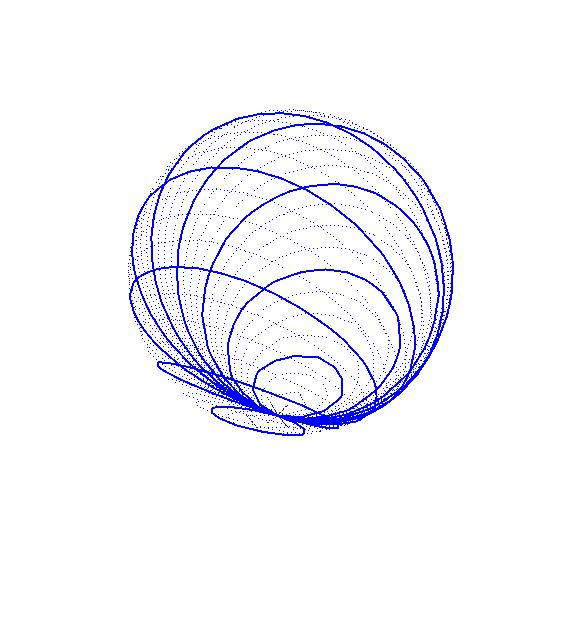
\includegraphics[trim=120 120 110 110, clip,scale=0.25]{omega2}
\end{figure}\\ %%%%%%%%%%%%%%%%%%%%%%%%%%%%%%%%%%%%%%%%%%%%%%%%%%%%%%%%%%%%%%%%%%%%%%%%
y por esto tiene sentido definir $\Omega^2Y:=\text{Map}_*(\Sn^2,Y)$.

Otra forma de verificar (\ref{eq:esfera_omega_adjuntas}) es con el siguiente ejercicio:

\import{\directory}{ejercicios/13} %%%%%%%%%%%%%%%%%%%%%%%%%%%%%%%%%%%%%%%%%%%%%% EJERCICIOS 13

Este ejercicio y (\ref{def:omega_n}) nos implica que:

\begin{cor}
  \[
    \pi_n(X,x_0)\cong\pi_0(\Omega^nX,x_0)\cong\pi_n(\text{Map}_*(\Sn^n,X))
  \]
\end{cor}

\end{document}